\section{Error Handling}
\label{error-handling-chap}
Error Handling is a vital general tool, which is used for the users to get an overview of the errors, which they made during their time coding the Ezuino programming language. The error handling tool is a part of the ANTLR V4 Runtime library, which uses its error handler as an interface which deal with syntax errors, which get encountered during the parsing of the ANTLR generated parse files. \\
\\
First, we use the ANTLRErrorListener class, which is an interface implementing methods for the different errors, the user may make during the program. The listener can report anything from syntax errors to ambiguity reports.
\begin{figure}[H]
\centering
\frame{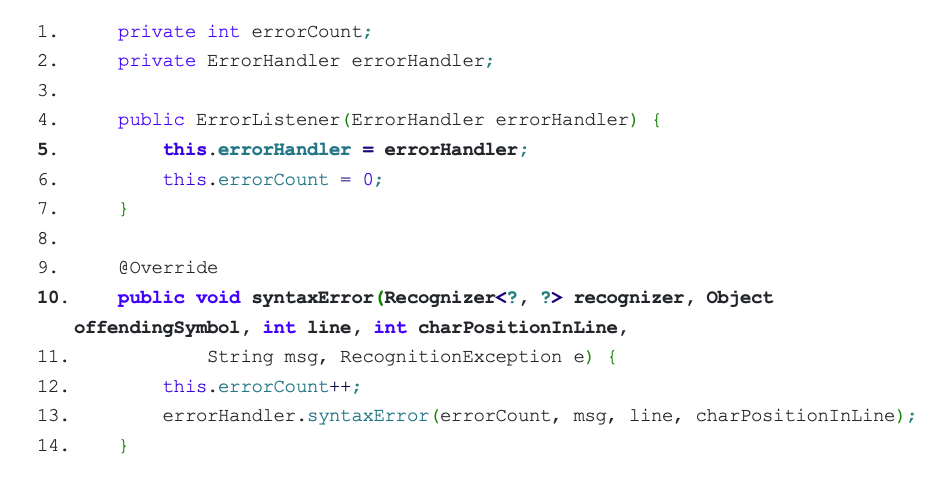
\includegraphics[scale=0.42]{figures/implementation/eh01.png}}
\caption{}
\label{eh01}
\end{figure}
The one we’re interested in is shown in figure \ref{eh01}. In this code, we’re inside the ErrorListener class, which implements the ANTLRErrorListener interface.  In figure \ref{eh01}, we got two global variables, errorCount, which is used to count the number of errors, ANTLR found during the parsing. The ErrorHandler instantiation is from the ErrorHandler class, which handles a specific type of errors during the AST, and covers more abstract error handling, for example, cast exceptions, type exceptions and many more. The ErrorHandler class will be described later in this section. \\
\\
The only method we are interested in is the syntaxError method, which is recognizing syntax errors made by the users. As an example, if the users input the code (int int), this would be a violation of the ANTLR grammar, as it’s two literals, the scanner review as int type declarations, without any ID after both the declarations. If the scanner recognizes this error, it will not run the visitors, or future visitors through, as the error was caught in the earlier stages of the process.
\begin{figure}[H]
\centering
\frame{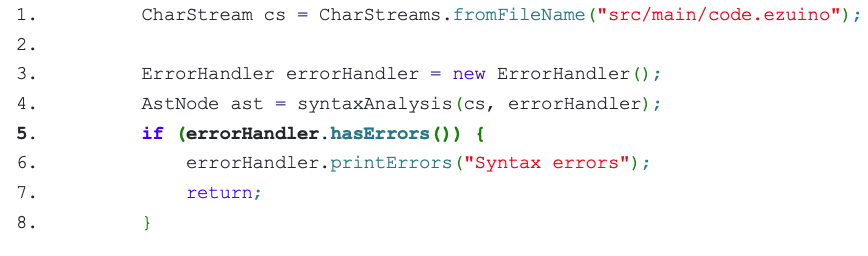
\includegraphics[scale=0.45]{figures/implementation/eh02.png}}
\caption{}
\label{eh02}
\end{figure}
Figure \ref{eh02}, is from the Main class in the Ezuino program. This class executes all the lexers, parsers, visitors, error handlers in order, to provide flow in the compile process. On figure \ref{eh02} in line 1, we use a character stream to read the written Ezuino program file from the code.ezuino file. We then create a new error handler, which we use the syntax analysis method to go through the parser and lexer file generated by ANTLR from the Ezuino grammar file. \\
\\
Going back to the ErrorHandler class, we got 3 methods, which has the main functionality of the error handler. 
\begin{figure}[H]
\centering
\frame{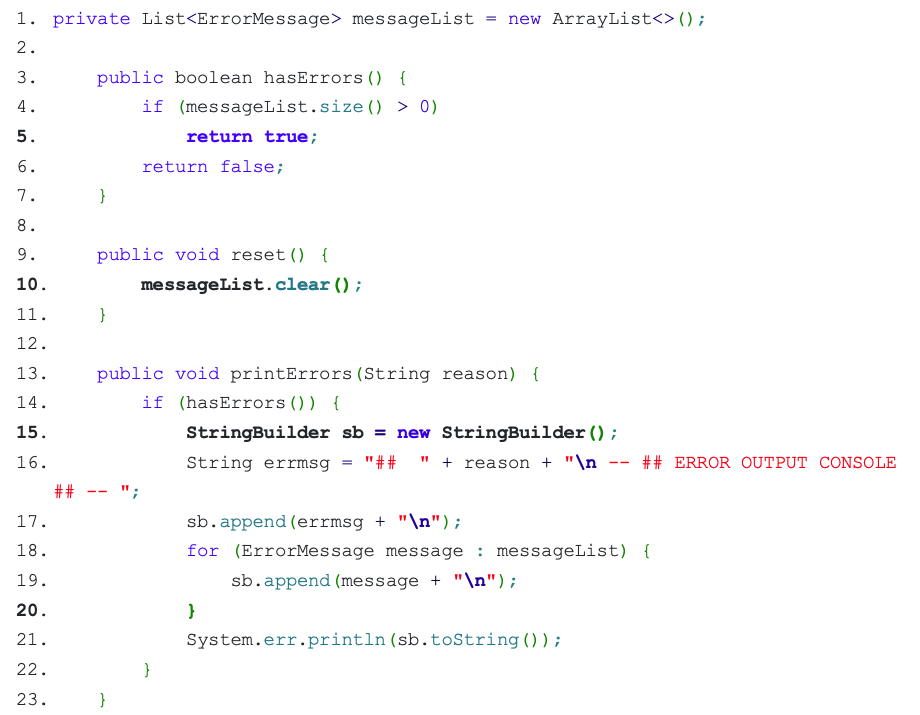
\includegraphics[scale=0.45]{figures/implementation/eh03.png}}
\caption{}
\label{eh03}
\end{figure}
Figure \ref{eh03}, is a snippet from the ErrorHandler class. On line 1, we got an ArrayList, which contains all the error messages found during the contextual analysis, reported by errors in the AST visitor classes. The method hasErrors() from line 3, checks the ArrayList mentioned in line 1, for its size, which means that the error handler has added an error to the error list. The reset() method on line 9, is used for the JUnit tests, which must reset its error handler for each test so that they do not overlap. Finally, from line 13 we got the printErrors() method, which prints the methods, which is in figure \ref{eh04}. First, it checks whenever there are errors, then it prints all the messages in the ArrayList, by running a for each loop for 18. 
\begin{figure}[H]
\centering
\frame{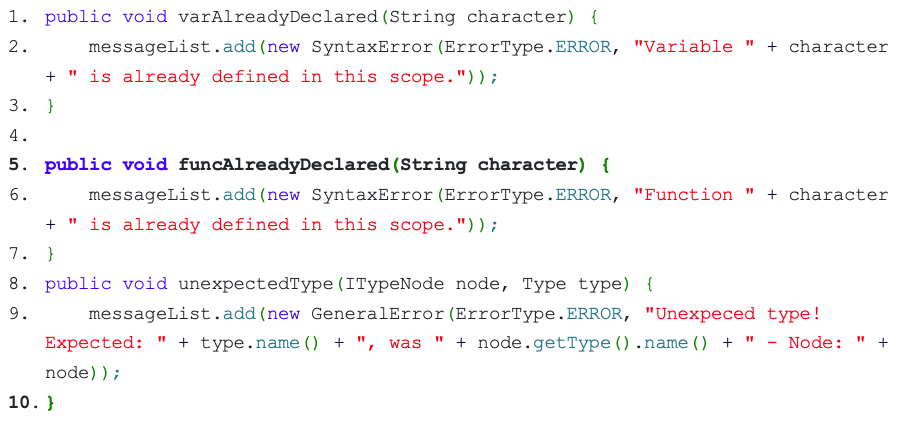
\includegraphics[scale=0.45]{figures/implementation/eh04.png}}
\caption{}
\label{eh04}
\end{figure}
Figure \ref{eh04} has 3 methods, which is being used within the visitors. The methods take either string as ID’s, or nodes and do in-method conversions of messages, which are being added to the ArrayList on figure \ref{eh03}, line 1. The SyntaxError and GeneralError classes both contain different string representations of each error. 
\begin{figure}[H]
\centering
\frame{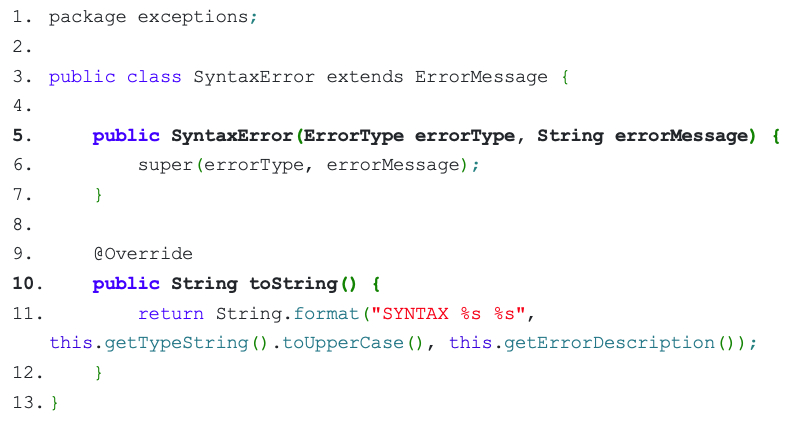
\includegraphics[scale=0.45]{figures/implementation/eh05.png}}
\caption{}
\label{eh05}
\end{figure}
Figure \ref{eh05} is an example of the SyntaxError class, for every error method in Figure \ref{eh04}, which constructs a new SyntaxError, will need the input of an Error Type and Error Message. Then, the toString() method from line 10, returns a string with a specific format, for this syntax error. 
To get an overview of these classes together, a relationship diagram has been created and can be reviewed in figure \ref{eh06} below.
\begin{figure}[H]
\centering
\frame{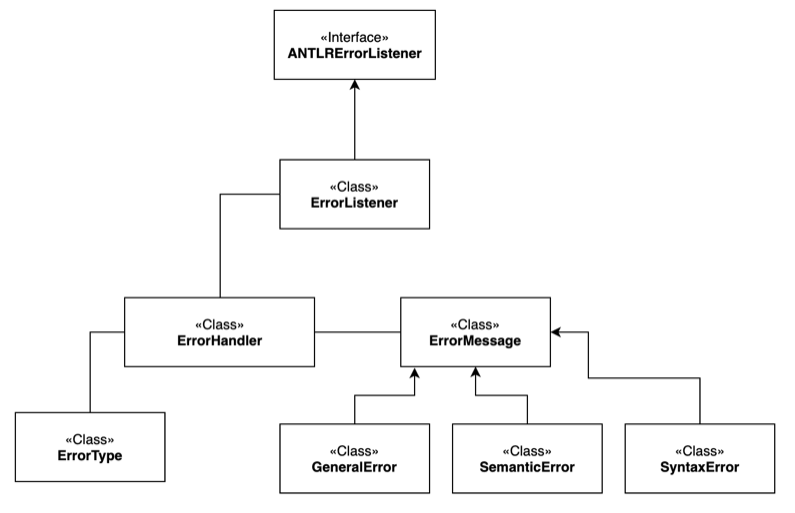
\includegraphics[scale=0.45]{figures/implementation/eh06.png}}
\caption{}
\label{eh06}
\end{figure}